\section{The bag of words and term-document matrix}
\label{sec:dtm}

Before you can analyse text using the computer, the text must be represented in a way that is understandable for the computer.

The Document-term matrix (DTM, also called the term-document matrix or TDM) is a common numerical representation of text.
This represents a \concept{corpus} (or set of documents) as a matrix or table, where each row represents a document, each column represents a term (word),
and the numbers in each cell show how often that word occurs in that document.

\pyrex[caption=Example document-term matrix,output=r,format=table]{ch_dtm/dtm}

As an example, \refex{dtm} shows a DTM made from two lines from the famous poem by Mary Angelou.
The resulting matrix has two rows, one for each line; and 11 columns, one for each unique term (word).
In the columns you see the document frequencies of each term: the word ``bird'' occurs once in each line,
but the word ``with'' occurs only in the first line (text1) and not in the second (text2).

In R, you can use the \fn{dfm} function from the \pkg{quanteda} package.
This function can take a vector or column of texts and transforms it directly into a DTM.
In Python, you achieve the same by creating an object of the \cls{CountVectorizer} class, which has a \fn{fit\_transform} function.


\subsection{Tokenization}

In order to turn a corpus into a matrix, each text needs to be \concept{tokenized},
meaning that it must be split into a list (vector) of words.
This seems trivial, as English (and most western) text generally uses spaces to demarcate words.
However, even for English there are a number of edge cases. 
For example, should `haven't' be seen as a single word, or two?

\pyrex[caption=Differences between tokenizers]{ch_dtm/tokenize}

\refex{tokenize} shows how Python and R deal with the sentence ``I haven't seen John's derring-do''.
For Python, we first use |CountVectorizer.build_tokenizer| to access the built-in tokenizer.
As you can see in the first line of input, this tokenizes ``haven't'' to |haven|,
which of course has a radically differeny meaning. Moreover, it silently drops all single-letter words,
including the |'t|, |'s|, and |I|.
A more reasonable tokenizer is the \cls{TreebankWordTokenizer} included in the \pkg{nltk} package, which contains a number of functions for doing natural language processing in python.
This tokenizer splits ``haven't'' into |have| and |n't|, which is a reasonable outcome.
Unfortunately, this tokenizer assumes that text has already been split into sentence,
and it also includes punctuation as tokens by default.
For this reason, we introduce a custom tokenizer based on the Treebank tokenizer,
which splits text into sentences (using \fn{nltk.sent\_tokenize}) and allows for a custom criterion for keeping tokens,
in this case that the token must contain at least one letter. 

For R, we simply call the \fn{tokens} function from the \quanteda\ package.
This keeps |haven't| and |John's| as a single word, which is probably less desirable than splitting the words
but at least better than outputting the word |haven|.

As this simple example shows, even a relatively simple sentence is tokenized differently by the three tokenizers considered here.
Depending on the research question, these differences might or might not be important.
However, it is always a good idea to check the output of this (and other) preprocessing steps so you understand
what information is kept or discarded.

% Listings won't work with the japanese output, so I manually created png. Sorry!
\begin{ccsexample}
  \doublecodex{ch_dtm/haiku}
  \begin{tcbraster}[raster columns=2,raster equal height=rows,raster valign=top]
  \begin{tcolorbox}[title=Python Output]
      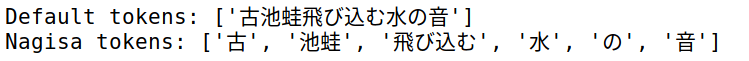
\includegraphics[width=\linewidth]{{ch_dtm/haiku.py}.png}
  \end{tcolorbox}%
  \begin{tcolorbox}[title=R Output]
      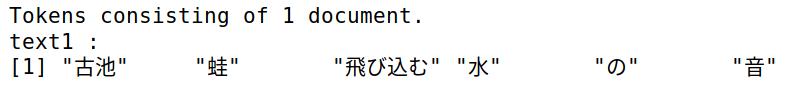
\includegraphics[width=\linewidth]{{ch_dtm/haiku.r}.png}
  \end{tcolorbox}%
\end{tcbraster}
  \caption{Tokenization of Japanese verse}\label{ex:haiku}
\end{ccsexample}



Note that for languages such as Chinese, Japanese, and Korean, which do not use spaces to delimit words, the story is more difficult.
Although a full treatment is beyond the scope of this book, \refex{haiku} shows a small example of tokenizing Japanese text,
in this case the famous haiku ``the sound of water'' by Bash\={o}.
The default tokenizer in quanteda actually does a good job, in contrast to the default python tokenizer
that simply keeps the whole string as one word
(which makes sense since this tokenizer only looks for whitespace or punctuation).
For python the best bet is to use a custom package for tokenizing Japanese, such as the \pkg{nagisa} package.
This package contains a tokenizer which is able to tokenize the Japanese text, and we could use this in the \cls{CountVectorizer}
much like we used the \cls{TreebankWordTokenizer} for English earlier.
Similarly, with heavily inflected languages such as Hungarian or Arabic,
it might be better to use preprocessing tools developed specifically for these languages, but treating those is unfortunately
beyond the scope of this book. 


\subsection{The DTM as a Sparse Matrix}

\pyrex[caption=Example document-term matrix]{ch_dtm/sotu}

\refex{sotu} shows a more realistic example.
It downloads all US 'State of the Union' speeches and creates a document-term matrix from them.
Since the matrix is now easily too large to print, both python and R simply list the size of the matrix.
R lists $85$ documents (rows) and $17,999$ features (columns), and Python reports that it's size is $85\times22219$.
Note the difference in the amount of columns (unique terms) due to the differences in tokenization as discussed above. 

\pyrex[caption=A look inside the DTM]{ch_dtm/freq}
\pyrex[caption=A look inside the DTM]{ch_dtm/freq2}

In \refex{freq} we show how you can look at the contents of the DTM. First, we show the overall term and document frequencies of each word, where we showcase words at different frequencies. Unsurprisingly, the word \emph{the} tops both charts, but further down there are minor differences.
In all cases, the highly frequent words are mostly functional words like \emph{them} or \emph{first}. More informative words such as \emph{investments} are by their nature used much less often.
Such term statistics are very useful to check for noise in the data and get a feeling of the kind of language that is used. 
Second, we take a look at the frequency of these same words in four speeches from Truman to Obama. All use words like \emph{the} and \emph{first}, but none of them talk about \emph{defrauded} -- which is not surprising, since it was only used once in all the speeches in the corpus.

However, the words that ranked around 1,000 in the top frequency are still used in less than half of the documents.
Since there are about 17,000 even less frequent words in the corpus, you can imagine that most of the document-term matrix consists of zeroes. 
The output also noted this \concept{sparsity} in the first output above.
In fact, R reports that the dtm is $91\%$ sparse, meaning that percentage of all entries is zero.
Python reports a similar figure, namely that there are only just under 150 thousand non-zero entries
out of a possible $8\times22219$, which boils down to a 92\% sparse matrix.

Note that to display the matrix we turned it from a \concept{sparse matrix} representation into a \concept{dense matrix}.
Briefly put, in a dense matrix, all entries are stored as a long list of numbers, including all the zeroes.
In a sparse matrix,  only the non-zero entries and their location are stored. 
This conversion (using the function \verb|as.matrix| and \verb|todense| respectively), however, was only performed after selecting a small subset of the data.
In general,  it is very inefficient to store and work with the matrix in a \concept[dense matrix]{dense} format.
For a reasonably large corpus with tens of thousands of documents and different words, this can quickly run billions of numbers,
which can cause problems even on modern computers and is moreover very inefficient.
With sparsities of often above 99\%, using a sparse matrix representation can easily reduce storage requirements by a hundred times and in the process speed up calculations by reducing the number of entries that need to be inspected.
Both \quanteda\ and \sklearn\ store DTMs as sparse matrices by default,
and most analysis tools are able to deal with sparse matrices very efficiently.
(but see \refsec{workflow} for problems with machine learning on sparse matrices in R). 

A final note on the difference between python and R in this example.
The code in R is much simpler and produces nicer results since it also shows the words and the speech names.
In python, we wrote our own helper function to create the frequency statistics which is built into the R \quanteda\ package.
These differences between Python and R reflect a pattern that is true in many (but not all) cases:
In python libraries such as \numpy\ and \sklearn\ are setup to maximize performance,
while in R a library such as \quanteda\ or \tidyverse\ is more geared towards ease of use.
For that reason, the DTM in python does not `remember' the actual words, it uses the index of each word,
so it consumes less memory if you don't need to use the actual words in e.g. a machine learning setup.
R, on the other hand, stores the words and also the document IDs and metadata in the DFM object.
This is easier to use if you need to look up a word or document, but it consumes (slightly) more memory. 


\begin{feature}
  \textbf{R: Why is it a document-feature matrix?}
The package \pkg{quanteda} uses the term document-feature matrix because the columns can also contain
other information instead of terms, such as word pairs, and these are collectively called \emph{features} of the text.
\end{feature}

\begin{feature}
\noindent\textbf{Python: Why fit\_transform?}
In Python, you don't have a function that directly transforms text into a DTM.
Instead, you create an \emph{transformer} called a CountVectorizer,
which can then be used to 'vectorize' texts (turn it into a row of numbers)
by counting how often each word occurs.
This uses the \fn{fit\_transform} function which is offered by all \sklearn\ transformers.
It `fits' the model on the training data, which in this case means learning the vocabulary.
It can then be used to transform other data into a DTM with the exact same columns,
which is often required for algorithms.
Because the feature names (the words themselves) are stored in the CountVectorizer
rather than the document-term matrix, you generally need to keep both objects.
\end{feature}

\subsection{The DTM as a `bag of words'}


As you can see already in these simple examples, the document-term matrix discards quite a lot of information from text.
Specifically, it disregards the order or words in a text: `John fired Mary' and `Mary fired John' both result in the same DTM,
even though the meaning of the sentences is quite different.
For this reason, a DTM is often called a \concept{bag of words}, in the sense that all words in the document are simply put in a big bag
without looking at the sentences or context of these words. 

Thus, the DTM can be said to be a specific and `lossy' representation of the text, that turns out to be quite useful for certain tasks:
The frequent occurrence of words like ``employment'', ``great'', or ``I'' might well be good indicators that a text is about the economy,
is positive, or contains personal expressions respectively.
As we will see in the next chapter, the DTM representation can be used for many different text analyses, from dictionaries to supervised and unsupervised machine learning.

Sometimes, however, you need information that is encoded in the order of words.
For example, in analysing conflict coverage it might be quite important to know who attacks whom, not just that attacking took place.
In the last section of this chapter we will look at some ways to create a richer matrix-representation by using word pairs.
Although it is beyond the scope of this book,
you can also use automatic syntactic analysis to take grammatical relations into account as well.
As is always the case with automatic analyses, it is important to understand what information the computer is looking at,
as the computer cannot find patterns in information that it doesn't have.

\subsection{The (unavoidable) Word Cloud}

One of the most famous text visualizations is without doubt the word cloud.
Essentially, a word cloud is an image where each word is displayed in a size that is representative of its frequency.
Depending on preference, word position and colour can be random, depending on word frequency, or in a decorative shape.

Word Clouds are often criticised since they are (sometimes) pretty but mostly not very informational.
The core reason for that is that only a single aspect of the words is visualized (frequency),
and simple word frequency is often not that informative: the most frequent words are generally uninformative `stop words' like ``the'' and ``I''.

For example, \refex{wordcloud} shows the word cloud for the state of the union speeches downloaded above.
In R, this is done using the \quanteda\ function \fn{textplot\_wordcloud}.
In Python we need to work a little harder, since it only has the counts, not the actual words.
So, we sum the DTM columns to get the frequency of each word, and combine that with the feature names (words)
from the |CountVectorized| object |cv|. Then we can create the WordCloud and give it the frequencies to use.
Finally, we plot the cloud and remove the axes.

\pyrex[caption=Word Cloud of the US State of the Union corpus,format=png]{ch_dtm/wordcloud}

The results from Python and R look different at first -- for one thing, R is nice and round but Python has more colors!
However, if you look at the cloud you can see both are not very meaningful: the largest words are all punctuation or words like
`a', `and', or `the'.
You have to look closely to find words like `federal' or `security' that give a hint on what the texts were actually about.


